\documentclass[tikz,border=8pt]{standalone}
\usetikzlibrary{arrows.meta}
\begin{document}
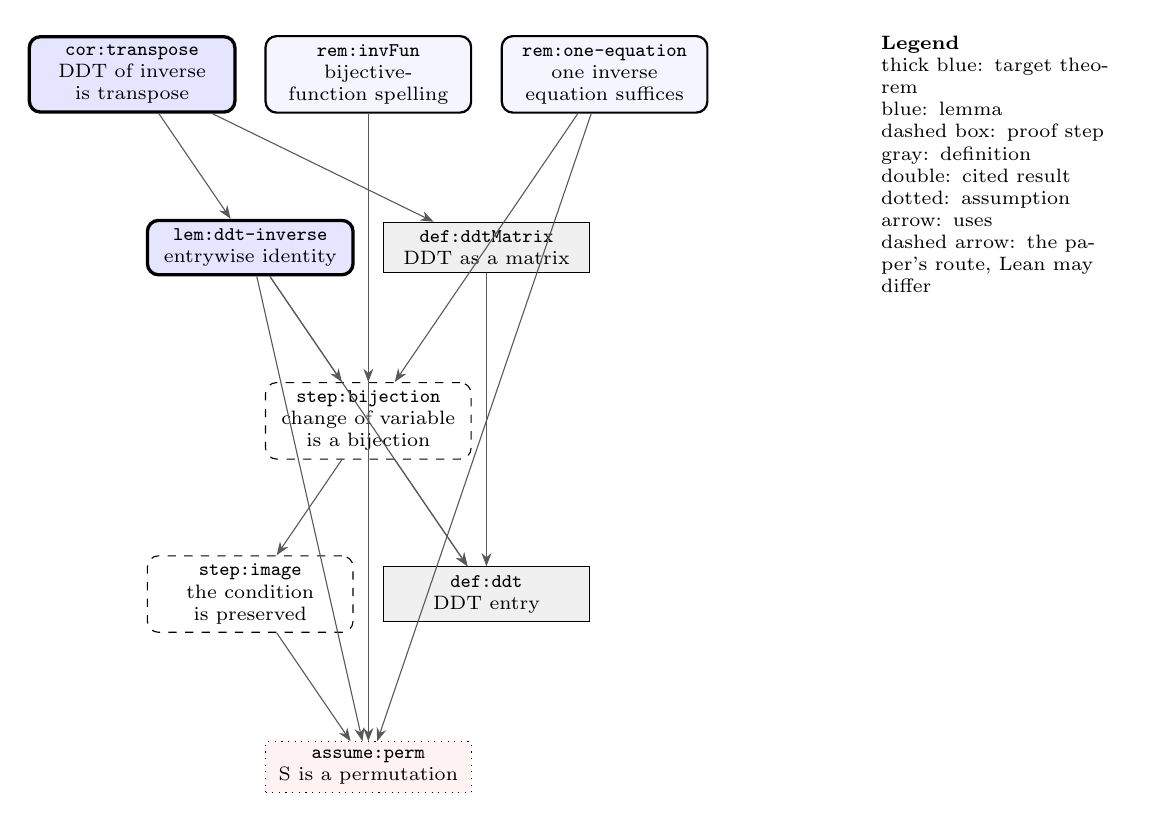
\begin{tikzpicture}[>=Stealth, every node/.style={font=\scriptsize, align=center, text width=2.4cm, inner sep=3pt}]
\node[draw, very thick, rounded corners, fill=blue!10] (cortranspose) at (-3.00,0.00) {\texttt{cor:transpose}\\DDT of inverse is transpose};
\node[draw, thick, rounded corners, fill=blue!4] (reminvFun) at (0.00,0.00) {\texttt{rem:invFun}\\bijective-function spelling};
\node[draw, thick, rounded corners, fill=blue!4] (remoneequation) at (3.00,0.00) {\texttt{rem:one-equation}\\one inverse equation suffices};
\node[draw, very thick, rounded corners, fill=blue!10] (lemddtinverse) at (-1.50,-2.20) {\texttt{lem:ddt-inverse}\\entrywise identity};
\node[draw, fill=gray!12] (defddtMatrix) at (1.50,-2.20) {\texttt{def:ddtMatrix}\\DDT as a matrix};
\node[draw, dashed, rounded corners] (stepbijection) at (0.00,-4.40) {\texttt{step:bijection}\\change of variable is a bijection};
\node[draw, dashed, rounded corners] (stepimage) at (-1.50,-6.60) {\texttt{step:image}\\the condition is preserved};
\node[draw, fill=gray!12] (defddt) at (1.50,-6.60) {\texttt{def:ddt}\\DDT entry};
\node[draw, dotted, fill=red!5] (assumeperm) at (0.00,-8.80) {\texttt{assume:perm}\\S is a permutation};
\draw[->, gray!70!black] (cortranspose) -- (lemddtinverse);
\draw[->, gray!70!black] (cortranspose) -- (defddtMatrix);
\draw[->, gray!70!black] (lemddtinverse) -- (stepbijection);
\draw[->, gray!70!black] (lemddtinverse) -- (defddt);
\draw[->, gray!70!black] (lemddtinverse) -- (assumeperm);
\draw[->, gray!70!black] (reminvFun) -- (stepbijection);
\draw[->, gray!70!black] (reminvFun) -- (assumeperm);
\draw[->, gray!70!black] (remoneequation) -- (stepbijection);
\draw[->, gray!70!black] (remoneequation) -- (assumeperm);
\draw[->, gray!70!black] (stepbijection) -- (stepimage);
\draw[->, gray!70!black] (stepbijection) -- (defddt);
\draw[->, gray!70!black] (stepimage) -- (assumeperm);
\draw[->, gray!70!black] (defddtMatrix) -- (defddt);
\node[anchor=north west, text width=3.2cm, font=\scriptsize, align=left] at (6.40,0.6) {\textbf{Legend}\\ thick blue: target theorem\\ blue: lemma\\ dashed box: proof step\\ gray: definition\\ double: cited result\\ dotted: assumption\\ arrow: uses\\ dashed arrow: the paper's route, Lean may differ};
\end{tikzpicture}
\end{document}
